% Slide 16 — Experimento 2: Bahia
\begin{frame}{Experimento 2: expansão na Bahia}
  \begin{columns}[T,onlytextwidth]
    \column{0.42\textwidth}
      \textbf{Escopo}
      \small
      \begin{itemize}
        \item 145 séries (loja, produto)
        \item 3 filiais, 6 segmentos comerciais
        \item 12 políticas $\times$ 5 replicações
        \item 8.700 pontos de avaliação
        \item Regime \textit{Lumpy} (71\% das séries)
      \end{itemize}
    \column{0.58\textwidth}
      \centering
      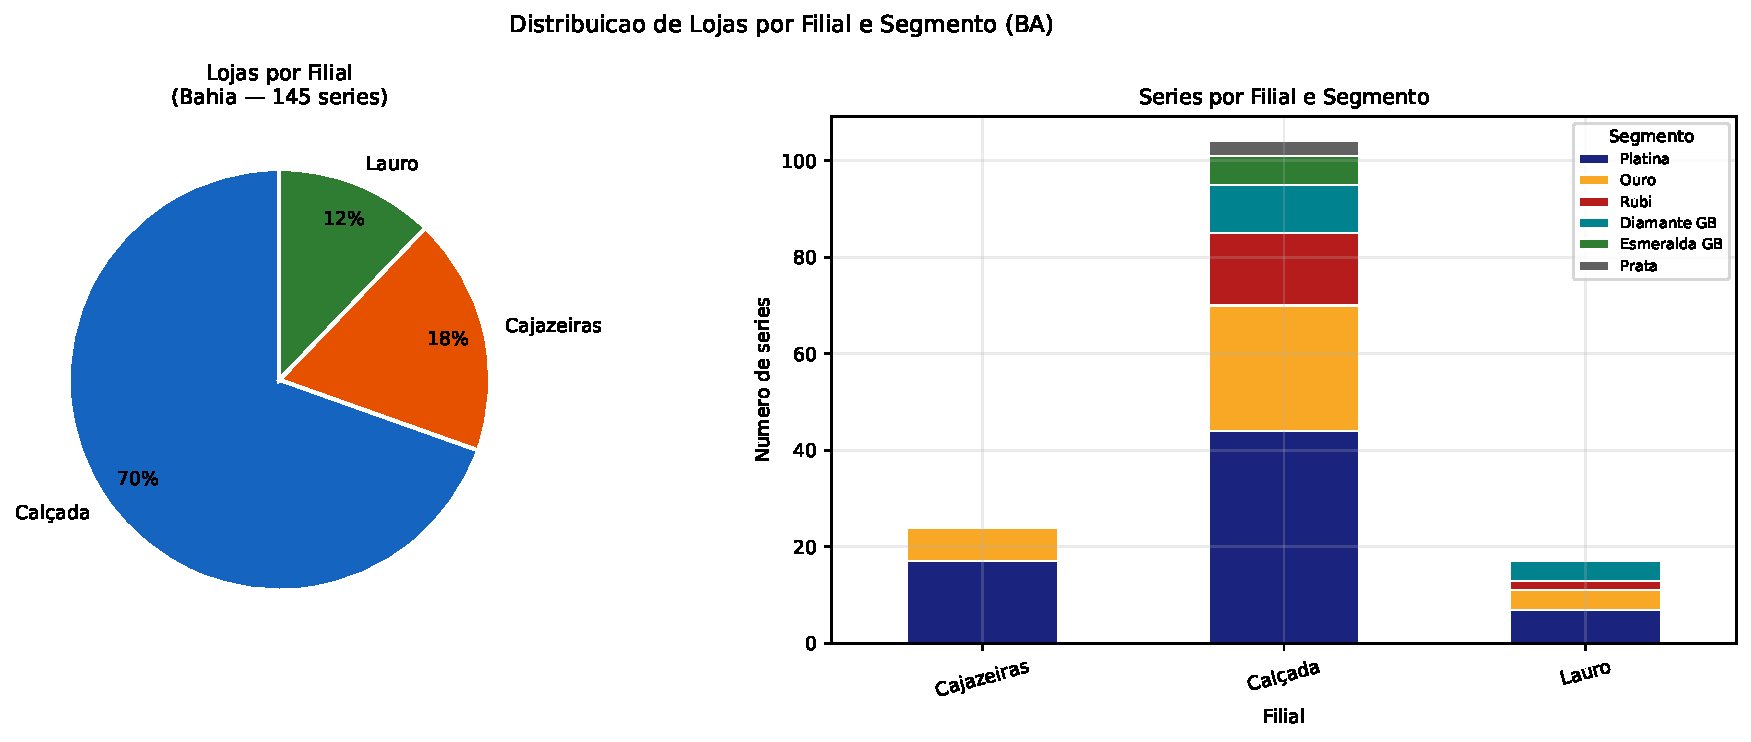
\includegraphics[width=\linewidth]{figures/distribuicao_lojas_segmento.pdf}
  \end{columns}
  \vspace{0.3em}
  \small \fonte{simulation/data/08\_reporting/maps/distribuicao\_lojas\_segmento}
  \note{
    O Experimento 2 amplia a escala: 145 combinações loja-produto do estado
    da Bahia, com cinco replicações independentes por política, totalizando
    8.700 pontos de avaliação. Isso habilita testes estatísticos formais,
    algo que o piloto da Paraíba não permitia com apenas uma replicação.
    A figura mostra como essas séries se distribuem entre as três filiais
    e os seis segmentos comerciais da rede -- a filial Calçada concentra
    72% das séries, o que é importante para interpretar os resultados
    agregados que vêm a seguir.
  }
\end{frame}
